\documentclass[output=paper]{langsci/langscibook} 
\title{The syntactic structure of negation in Ndebele} 
\author{%
 Ross Burkholder \affiliation{University of Chicago}
}
% \chapterDOI{} %will be filled in at production

\newcommand{\nga}[0]{\textit {-nga- }}
\newcommand{\ii}[0]{\textit {-i- }}
\newcommand{\ka}[0]{\textit {-(k)a- }}
\newcommand{\bee}[0]{\textit {be }}

\abstract{
This paper closely examines the structure of negation in Ndebele, a Bantu language spoken in Zimbabwe. The paper argues for the presence of a null verbal element which occurs in some types of Ndebele clauses. In addition the claim is made that the two pieces of Ndebele bipartite negation are realizations of two different nodes, a higher NegP node and a lower TP node which is sensitive to polarity. There are two primary pieces of evidence in favor of this hypothesis. The first is that adopting such a structure allows us to treat the negative prefix \nga and the negative suffix \textit{-anga-} as a single morpheme, contrary to current proposals (Buell 2004; 2005; Khumalo 1981; 1982; Sibanda 2004). A second piece of evidence is that introducing a null verbal element where proposed provides an explanation for previously unaccounted for data in the realm of adjectival predicates.}

\maketitle
\begin{document}


%% ----------------------------------------------------------------------------%
%% ----------------------------------------------------------------------------%

 

  

\section{Introduction and background}

This paper closely examines the structure of negation in Ndebele,\footnote{Guthrie Code: S.44} a Bantu language spoken in Zimbabwe. The paper argues for the presence of a null verbal element which occurs in some types of Ndebele clauses. In addition, the claim is made that the two pieces of Ndebele bipartite negation are realizations of two different nodes, a higher NegP node and a lower TP node which is sensitive to polarity. There are two primary pieces of evidence in favor of this hypothesis. The first is that adopting such a structure allows us to treat the negative prefix \nga and the negative suffix \textit{-anga-} as a single morpheme, contrary to current proposals (Buell 2004; 2005;\footnote{Buell (2004) and (2005) make this argument for Zulu, an extremely closely related language. For the purposes of this argument the two languages seem to function identically; thus, the claims made here apply to both languages unless otherwise specified.} Khumalo 1981; 1982; Sibanda 2004). A second piece of evidence is that introducing a null verbal element where proposed provides an explanation for previously unaccounted for data in the realm of adjectival predicates. \S1 will introduce necessary background information on the language.  \S2 will introduce our proposed clausal structure as it relates to the negation of simple tense verbal predicates. In addition \S2 will show how the distribution of negative morphemes in Ndebele can be accounted for via agreement with a series of binary features. \S3 will show how null verbal projections can be utilized to deal with both positive and negative adjectival predicates. \S4 extends the argument to imperatives. \S5 concludes the paper. 


\subsection{Background}

Negation in Ndebele shows a bipartite distribution, as demonstrated in (1).


\begin{exe}
\ex \gll  \textit{\textbf {ka}-ngi-pheg-\textbf{i}}\\
          {\sc neg}-1.{\sc sm}-cook-{\sc prs.neg}\\
    \glt `I do not cook'
\end{exe}


For this reason it will make sense to refer to negative affixes as either prefixal or suffixal, depending on their linear surface relation to the verb root. Thus it can be seen from (1) that \textit{ka-} is a negative prefix, while \ii is a negative suffix.\footnote{The negative affix \textit{ka-} can appear with or without the initial /k/ sound depending on context; thus, it is referred to as \textit{ka-} throughout.} The negative affix that we will be primarily describing in this paper, however, seems to behave differently from the two demonstrated in (1) in that it can appear as either a prefix or a suffix.

\begin{exe}
\ex \begin{xlist}
\ex \gll \textit{isi-lwane}  \textit{be-si-\textbf{nga}-nhle}\\
       7-lion {\sc cop}-7.{\sc sm}-{\sc pst.neg}-pretty\\
    \glt `The lion wasn't pretty' 

\ex \gll \textit{um-fana} \textit{ka-khal-a-\textbf{nga}}\\
         1-boy {\sc neg}-cry-{\sc ep}-{\sc pst.neg}\\
    \glt `The boy wasn't crying'
\end{xlist}
\end{exe}

The claim that the two negative morphemes in bold font in example (2) are the same morpheme is particular to this paper. In previous analyses these two morphemes are listed separately, with \textit{nga}- being listed as a negative prefix and -\textit{anga} being listed as a suffix (Sibanda 2004; Khumalo 1981; 1982).\footnote{In addition, the separation of suffixal \textit{-anga} into an epenthetic vowel \textit{-a-} and suffix \textit{-nga} is unique to this paper} The goal of this paper will be to show that not only is it possible to analyze the two morphemes in (2) as a single morpheme, but to show that in addition to being a simpler analysis, this analysis is also able to deal with previously unaccounted for data.

\section{Analysis of simple tense verbal predicates}

%This section outlines the system of Agree utilized in this paper. This system is then used to showcase the clausal structure proposed in this paper and how it can successfully be applied to %verbal predicates in the two simple tenses in Ndebele, present tense and recent past tense. This is done in order to demonstrate the functionality of the clausal structure, as well as %familiarize the reader with the general structure of Ndeble clauses. 


\subsection{Agree}

This analysis makes use of a system of Agree loosely based on the one described in Zeijlstra (2010). In his paper, Zeijlsta agrees with Boskovic (2007) that Agreement is unidirectional. Unlike Boskovic, however, Zeijlstra argues that this direction is upwards rather than downwards. Zeijlstra argues that one of the advantages of this this type of system is that it can account for patterns of negative concord by allowing several lower nodes to Agree with a single higher node without constituting a violation of relativized minimality (Rizzi 1989). It is this aspect of Zeijlstra's system which will be particularly useful to the analysis of negation in this paper. In this paper a middle ground is struck which preserves the heart of the Agreement system proposed by Zeijlstra and Boskovic, but which loosens the directionality requirement to one direction for a single instance of Agree, in general allowing both upward and downward agreement.

 Utilizing this analysis of Agree, the realizations of the polarity node can be determined by a series of binary features (Polarity, Past, Verbal) while the realization of tense nodes can be captured by a trinary feature (Tense) and two binary features (Neg, Verbal).

%\begin{figure}[ht!]
%\centering
%\includegraphics[width=90mm]{agreement.jpg}
%\caption{Upwards Agreement (Zeijlstra 2012)}
%\label{overflow}
%\end{figure}





\begin{exe}
\ex \textbf{Agree:} $\alpha$ can Agree with $\beta$ iff:


a. $\alpha$ carries at least one uninterpretable feature and $\beta$ carries a matching interpretable 

feature.


b. $\beta$ c-commands $\alpha$ OR $\alpha$ c-commands $\beta$.


c. $\beta$ is the closest goal to $\alpha$.
\end{exe}

As mentioned above, Ndebele has a bipartite system of negation. The claim made in this paper is that the higher of these two nodes is a true polarity projection, while the lower node is a tense node which is sensitive to polarity. The realizations for the polarity node, which is sensitive to the tense of the clause and whether or not the clause is verbal or nonverbal, are given below. In the tables below, the different realizations are given in the first row, and the featural distribution(s) which produce each of these realizations are given in the subsequent rows. Thus each column represents a featural distribution (pluses and minuses) whose morphological realization is the first row in that column. In Table 1, for example, the realization of the morpheme is null (shown in the first row) regardless of the featural distribution (the arrangement of pluses and minuses in each column beneath). This is not the case for the realizations of negative polarity shown in Table 2. In Table 2 there are two possible realizations depending of the featural distribution. Tables for the tense nodes will be given in the relevant sections.

%\begin{table}
%\caption{Realizations of Future Tense} %title of the table 
%\centering % centering table 
%\begin{tabular}{c| rrrr} % creating eight columns 
%\hline %inserting double-line 
%&\multicolumn{4}{c}{za} \\ [0.5ex] 
%\hline % inserts single-line 
%Neg & + & + & - & -\\ % Entering row contents 
%Verbal & + & - & +& -\\[1ex] % [1ex] adds vertical space 
%\hline % inserts single-line 
%\end{tabular} 
%\label{tab:hresult} 
%\end{table} 



\begin{table}
\caption{Realizations of Positive Polarity} %title of the table 
\centering % centering table 
\begin{tabular}{c| rrrr} % creating eight columns 
\hline %inserting double-line 
  &\multicolumn{4}{c}{$\emptyset$-} \\ [0.5ex] 
\hline % inserts single-line 
Past & + & + & - & -\\ % Entering row contents 
Verbal & + & - & +& -\\[1ex] % [1ex] adds vertical space 
\hline % inserts single-line 
\end{tabular} 
\label{tab:hresult} 
\end{table} 

\begin{table}
\caption{Realizations of Negative Polarity} %title of the table 
\centering % centering table 
\begin{tabular}{c| r|rrr} % creating eight columns 
\hline %inserting double-line 
 &\multicolumn{1}{c}{$\emptyset$-} &\multicolumn{3}{|c}{(k)a-} \\ [0.5ex] 
\hline % inserts single-line 
Past & + & + & - & -\\ % Entering row contents 
Verbal & - & + & +& -\\[1ex] % [1ex] adds vertical space 
\hline % inserts single-line 
\end{tabular} 
\label{tab:hresult} 
\end{table} 





%A discussion of the other tenses in Ndebele, distant past, near future, and distant future will be touched upon in section X which deals with complex tense %predicates.

\subsection{Present tense}

This section provides an introduction to the clausal structure proposed in this paper by showing how it accounts for simple present tense sentences such as those given in (4).
 

\begin{exe}
\ex \begin{xlist}
\ex \gll  \textit{ngi-pheg-a}\\
          1.{\sc sm}-cook-\sc prs\\
    \glt `I cook'


%Note: This is actually an unattested form, this form might need an object, otherwise it might need to be ngiyaphega



\ex \gll  \textit{\textbf{ka}}-\textit{ngi-pheg-\textbf{i}}\\
          {\sc neg}-1.{\sc sm}-cook-{\sc prs.neg}\\
    \glt `I do not cook'
\end{xlist}
\end{exe}
 

The realization of present tense morphemes is given in Table 3.

\begin{table}
\caption{Realizations of Present Tense} %title of the table 
\centering % centering table 
\begin{tabular}{c| r|r|rr} % creating eight columns 
\hline %inserting double-line 
 &\multicolumn{1}{c}{-i}& \multicolumn{1}{|c|}{-a}& \multicolumn{2}{|c}{-$\emptyset$} \\ [0.5ex] 
\hline % inserts single-line 
Neg & + & - & + & -\\ % Entering row contents 
Verbal & + & + & -& -\\[1ex] % [1ex] adds vertical space 
\hline % inserts single-line 
\end{tabular} 
\label{tab:hresult} 
\end{table} 


In other Bantu studies, the morpheme \textit{-a} found in (4a) is often glossed as a final vowel (Khumalo 1981; 1982; Sibanda 2004). In the analysis presented in this paper, however, it will be treated as tense node, as demonstrated both in Table 3 and the tree structures given in (5)-(8). Due to the abundance of Agreement and movement in the examples given, four tree structures are given, each of which highlights particular aspects of the tree. In (5)-(8), dotted lines are used to show Agreement, while solid lines are used to show overt movement. Arrows are used to show the direction of both movement and Agreement; thus a dotted line with arrows pointing in both directions shows Agreement between two nodes in both directions. Following Chomsky (2001), this analysis makes use of a distinction between interpretable and uninterpretable features. Uninterpretable features, demarcated by a `u' before the feature name, must be checked in order for the utterance to be grammatical. Uninterpretable features are checked when they Agree with a matching interpretable feature (demarcated by an `i' preceding the feature name). Strikethrough is used in (6) and (7) to show that uninterpretable features are checked. (5)  gives the underlying structure of the tree before Agree or movement have taken place. (6) shows how the proposed system of Agree works to successfully check all uninterpretable features, while (7) demonstrates movement of the verb from the V(erb) to the T(ense) node (V-T movement). (8) is a simplified tree structure representing (4a). This structure exemplifies the kind of simplified tree structure that will be utilized throughout the remainder of this paper where only the dotted lines of agreement are shown, and uninterpretable features do not use strikethrough even when checked so as to remain clear to the reader. Paths of movement can still be easily noted in the simplified tree structure by the placement of traces (t) coindexed with the lexical material.

 

\begin{exe}
\ex
\end{exe}
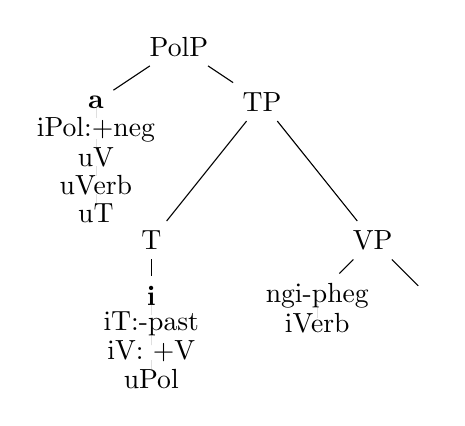
\begin{tikzpicture}[
sibling distance=6em,
level distance=2em]
\node (root) at (0,0) {PolP}
			child { node  {\textbf{a}} [sibling distance=8em, level distance=1em]
				child { node {iPol:+neg} [line width=.001mm, sibling distance=8em, level distance=1em]
					child { node {uV}
						child { node {uVerb}
							child { node (pol){uT}}}}}}
			child {node {TP}[sibling distance=8em, level distance=5em] 
				child { node {T}[sibling distance=4em, level distance=2em] 
					child { node {\textbf{i}}  [ sibling distance=8em, level distance=1em]
						child { node {iT:-past}  [line width=.001mm, sibling distance=8em, level distance=1em]
							child { node { iV: +V}
								child { node (t){uPol}}}}}}
				child { node {VP}[sibling distance=4em, level distance=2em] 
						child { node  {ngi-pheg}[sibling distance=8em, level distance=1em]
							child { node (V){iVerb} [line width=.001mm]}}
						child { node {}}}};
%\draw (V) [->]to[out=280,in=270] (vt);
%\draw[->, dashed] (pol) to[out=230,in=280] (c);

%\draw[<-, dashed] (t) to[out=230,in=280] (-2.3, -4);
%\draw[<-,dashed] (pol) to[out=230,in=100] (-2.3, -4);

%\draw[<-, dashed] (V) to[out=250,in=280] (-2.5,-4.5);
%\draw[dashed] (pol) to[out=200,in=100] (-2.5,-4.5);

%\draw[dashed] (t) to[out=250,in=280] (-2,-3);
%\draw[dashed] (c) to[out=220,in=100] (-2,-3);
\end{tikzpicture}


  


\begin{exe}
\ex
\end{exe}
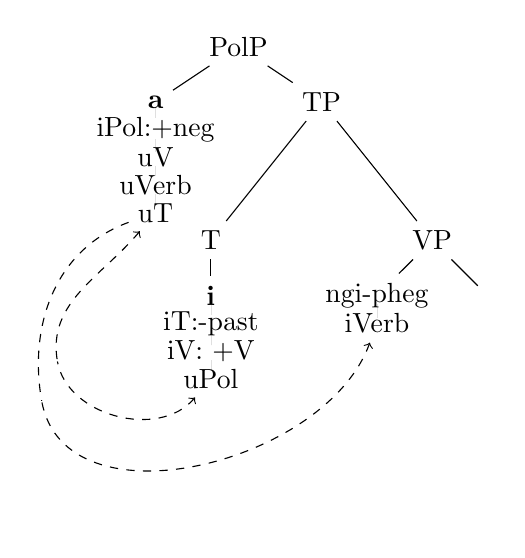
\begin{tikzpicture}[
sibling distance=6em,
level distance=2em]
\node (root) at (0,0) {PolP}
			child { node  {\textbf{a}} [sibling distance=8em, level distance=1em]
				child { node {iPol:+neg} [line width=.001mm, sibling distance=8em, level distance=1em]
					child { node {\st{uV}}
						child { node {\st{uVerb}}
							child { node (pol){\st{uT}}}}}}}
			child {node {TP}[sibling distance=8em, level distance=5em] 
				child { node {T}[sibling distance=4em, level distance=2em] 
					child { node {\textbf{i}}  [ sibling distance=8em, level distance=1em]
						child { node {iT:-past}  [line width=.001mm, sibling distance=8em, level distance=1em]
							child { node { iV: +V}
								child { node (t){\st{uPol}}}}}}}
				child { node {VP}[sibling distance=4em, level distance=2em] 
						child { node  {ngi-pheg}[sibling distance=8em, level distance=1em]
							child { node (V){iVerb} [line width=.001mm]}}
						child { node {}}}};
%\draw (V) [->]to[out=280,in=270] (vt);
%\draw[->, dashed] (pol) to[out=230,in=280] (c);

\draw[<-, dashed] (t) to[out=230,in=280] (-2.3, -4);
\draw[<-,dashed] (pol) to[out=230,in=100] (-2.3, -4);

\draw[<-, dashed] (V) to[out=250,in=280] (-2.5,-4.5);
\draw[dashed] (pol) to[out=200,in=100] (-2.5,-4.5);

%\draw[dashed] (t) to[out=250,in=280] (-2,-3);
%\draw[dashed] (c) to[out=220,in=100] (-2,-3);
\end{tikzpicture}
 


\begin{exe}
\ex
\end{exe}
\todo[inline]{tree commented out due to compile problems}
% \begin{tikzpicture}[
% sibling distance=6em,
% level distance=2em]
% \node (root) at (0,0) {PolP}
% 			child { node  {\textbf{a}} [sibling distance=8em, level distance=1em]
% 				child { node {iPol:+neg} [line width=.001mm, sibling distance=8em, level distance=1em]
% 					child { node {\st{uV}}
% 						child { node {\st{uVerb}}
% 							child { node (pol){\st{uT}}}}}}}
% 			child {node {TP}[sibling distance=8em, level distance=5em] 
% 				child { node {T}[sibling distance=4em, level distance=2em] 
% 					child { node (vt) {\textbf{ngi-pheg_i}} }
% 					child { node {\textbf{i}}  [ sibling distance=8em, level distance=1em]
% 						child { node {iT:-past}  [line width=.001mm, sibling distance=8em, level distance=1em]
% 							child { node { iV: +V}
% 								child { node (t){\st{uPol}}}}}}}
% 				child { node {VP}[sibling distance=4em, level distance=2em] 
% 						child { node  {t_i}[sibling distance=8em, level distance=1em]
% 							child { node (V){iVerb} [line width=.001mm]}}
% 						child { node {}}}};
% \draw (V) [->]to[out=280,in=270] (vt);
% %\draw[->, dashed] (pol) to[out=230,in=280] (c);
% 
% %\draw[<-, dashed] (t) to[out=230,in=280] (-2.3, -4);
% %\draw[<-,dashed] (pol) to[out=230,in=100] (-2.3, -4);
% 
% %\draw[<-, dashed] (V) to[out=250,in=280] (-2.5,-4.5);
% %\draw[dashed] (pol) to[out=200,in=100] (-2.5,-4.5);
% 
% %\draw[dashed] (t) to[out=250,in=280] (-2,-3);
% %\draw[dashed] (c) to[out=220,in=100] (-2,-3);
% \end{tikzpicture}













\begin{exe}
\ex
\end{exe}

\todo{tree commented out due to compile problems}

% \begin{tikzpicture}[
% sibling distance=6em,
% level distance=2em]
% \node (root) at (0,0) {PolP}
% 			child { node  {$\emptyset$} [sibling distance=8em, level distance=1em]
% 				child { node {iPol:-neg} [line width=.001mm, sibling distance=8em, level distance=1em]
% 					child { node {uT}
% 						child { node (pol){uV}}}}}
% 			child {node {TP}[sibling distance=8em, level distance=5em] 
% 				child { node {T}[sibling distance=4em, level distance=2em] 
% 					child { node (vt) {\textbf{ngi-pheg_i}} }
% 					child { node {\textbf{a}}  [ sibling distance=8em, level distance=1em]
% 						child { node {iT:-past}  [line width=.001mm, sibling distance=8em, level distance=1em]
% 							child { node { iV: +V}
% 								child { node (t){uPol}}}}}}
% 				child { node {VP}[sibling distance=4em, level distance=2em] 
% 						child { node  {t_i}[sibling distance=8em, level distance=1em]
% 							child { node (V){iVerb} [line width=.001mm]}}
% 						child { node {}}}};
% %\draw (V) [->]to[out=280,in=270] (vt);
% %\draw[->, dashed] (pol) to[out=230,in=280] (c);
% 
% \draw[<-, dashed] (t) to[out=230,in=280] (-2.3, -4);
% \draw[<-,dashed] (pol) to[out=230,in=100] (-2.3, -4);
% 
% %\draw[<-, dashed] (V) to[out=250,in=280] (-1.5,-4.5);
% %\draw[dashed] (pol) to[out=250,in=100] (-1.5,-4.5);
% 
% %\draw[dashed] (t) to[out=250,in=280] (-2,-3);
% %\draw[dashed] (c) to[out=220,in=100] (-2,-3);
% \end{tikzpicture}



 





The reasoning for positing that final vowels are generated under tense is as follows. First, both positive and negative realizations of the final vowel contribute semantically to tense. Indeed, in examples such as (4) they are the only overt markers of tense. Furthermore, the complementary distribution of final vowels and negative suffixes makes an argument which treats them as generated under separate nodes undesirable. The solution presented in this paper accounts for these facts by positing that final vowels and negative suffixes are both generated under a tense node which is sensitive to the polarity of the sentence as well as other clausal information (discussed further in \S3).

%This is not the only possible solution to this problem. It could also be argued that both final vowels and negative suffixes are generated in a final vowel node, which is itself sensitive to %polarity and tense, both of which could be generated higher in the clause. We will continue to posit the former analysis rather than the latter in this paper, partially due to the lack of %evidence of a true tense node other than the final vowel. However, distinguishing between such claims is not crucial to the claims made in this paper, and thus will largely be left to further %research.

Returning to the discussion of the simple present tense sentences in (4), the system of Agreement discussed in \S2.1 is demonstrated. As can be seen from the trees in (6) and (7), there are two primary nodes which participate in Agreement, PolP and TP. Each of these nodes is in an Agreement relationship with the other, and the Agreement relationship is largely symmetrical. Tense carries an interpretable tense feature as well as an interpretable feature which dictates whether the clause is verbal or nonverbal (+V or -V). The uninterpretable polarity feature on the tense node is checked by its Agreement relationship with PolP. PolP carries the interpretable feature polarity as well as two uninterpretable features, tense and uV, which is sensitive to whether or not the clause is verbal. Both of these uninterpretable features are checked by TP. Different realizations of these nodes are treated as separate lexical items, and thus can carry slightly different featural arrangements. Note that the negative polarity node also carries an uninterpretable uVerb feature (that positive polarity does not) which is checked by the verb. In verbal sentences this feature causes no distinguishable difference, and will thus be discussed in \S3 on adjectival predicates. In general relevant featural differences in the different realizations will be discussed in the corresponding sections. The Agreement relationship between PolP and TP will be a key component of the analysis presented here.


\subsection{Past tense}

The same analysis used for present tense clauses in \S2.2 directly applies to past tense clauses, as demonstrated in (9)-(11).



\begin{exe}
\ex \begin{xlist}
\ex \gll \textit{mina} \textit{ngi-khal-e}\\
         I 1.{\sc sm}-cry-{\sc pst}\\
    \glt `I was crying'


%Check if ka is actually the first person subject marker, this is an unattested form again that I made up


\ex \gll \textit{mina} \textit{a-ngi-khal-a-\textbf{nga}}\\
         I {\sc neg}-1.{\sc sm}-cry-{\sc ep}-{\sc pst.neg}\\
    \glt `I wasn't crying'
\end{xlist}
\end{exe}





\begin{table}
\caption{Realizations of Past Tense} %title of the table 
\centering % centering table 
\begin{tabular}{c| rr|r|r} % creating eight columns 
\hline %inserting double-line 
 &\multicolumn{2}{c}{-nga-}& \multicolumn{1}{|c}{-e-}& \multicolumn{1}{|c}{$\emptyset$} \\ [0.5ex] 
\hline % inserts single-line 
Neg & + & + & - & -\\ % Entering row contents 
Verbal & + & - & +& -\\[1ex] % [1ex] adds vertical space 
\hline % inserts single-line 
\end{tabular} 
\label{tab:hresult} 
\end{table} 


The sentences in (9) are quite similar to the present tense sentences in (4). The trees are provided in (10)-(11).




\begin{exe}
\ex
\end{exe}
\todo[inline]{Tree commented out due to compile problems}
% \begin{tikzpicture}[
% sibling distance=6em,
% level distance=2em]
% \node (root) at (0,0) {PolP}
% 			child { node  {$\emptyset$} [sibling distance=8em, level distance=1em]
% 				child { node {iPol:-neg} [line width=.001mm, sibling distance=8em, level distance=1em]
% 					child { node {uT}
% 						child { node (pol){uV}}}}}
% 			child {node {TP}[sibling distance=8em, level distance=5em] 
% 				child { node {T}[sibling distance=4em, level distance=2em] 
% 					child { node (vt) {\textbf{ngi-khal_i}} }
% 					child { node {\textbf{e}}  [ sibling distance=8em, level distance=1em]
% 						child { node {iT:+past}  [line width=.001mm, sibling distance=8em, level distance=1em]
% 							child { node { iV: +V}
% 								child { node {uPol}
% 									child { node (t){uVerb}}}}}}}
% 				child { node {VP}[sibling distance=4em, level distance=2em] 
% 						child { node  {t_i}[sibling distance=8em, level distance=1em]
% 							child { node (V){iVerb} [line width=.001mm]}}
% 						child { node {}}}};
% %\draw (V) [->]to[out=280,in=270] (vt);
% \draw (V) [<-, dashed]to[out=280,in=270] (t);
% %\draw[->, dashed] (pol) to[out=230,in=280] (c);
% 
% \draw[<-, dashed] (t) to[out=230,in=280] (-2.3, -4);
% \draw[<-,dashed] (pol) to[out=230,in=100] (-2.3, -4);
% 
% %\draw[<-, dashed] (V) to[out=250,in=280] (-2.25,-5.5);
% %\draw[dashed] (pol) to[out=200,in=100] (-2.25,-5.5);
% 
% %\draw[dashed] (t) to[out=250,in=280] (-2,-3);
% %\draw[dashed] (c) to[out=220,in=100] (-2,-3);
% \end{tikzpicture}





\begin{exe}
\ex
\end{exe}

\todo[inline]{Tree commented out due to compile problems}

% \begin{tikzpicture}[
% sibling distance=6em,
% level distance=2em]
% \node (root) at (0,0) {PolP}
% 			child { node  {a} [sibling distance=8em, level distance=1em]
% 				child { node {iPol:+neg} [line width=.001mm, sibling distance=8em, level distance=1em]
% 					child { node {uT}
% 						child { node {uV}
% 							child { node (pol){uVerb}}}}}}
% 			child {node {TP}[sibling distance=8em, level distance=5em] 
% 				child { node {T}[sibling distance=4em, level distance=2em] 
% 					child { node (vt) {\textbf{ngi-khal_i}} }
% 					child { node {\textbf{a-nga}}  [ sibling distance=8em, level distance=1em]
% 						child { node {iT:+past}  [line width=.001mm, sibling distance=8em, level distance=1em]
% 							child { node { iV: +V}
% 								child { node {uPol}
% 									child { node (t){uVerb}}}}}}}
% 				child { node {VP}[sibling distance=4em, level distance=2em] 
% 						child { node  {t_i}[sibling distance=8em, level distance=1em]
% 							child { node (V){iVerb} [line width=.001mm]}}
% 						child { node {}}}};
% %\draw (V) [->]to[out=280,in=270] (vt);
% \draw (V) [<-, dashed]to[out=280,in=270] (t);
% %\draw[->, dashed] (pol) to[out=230,in=280] (c);
% 
% \draw[<-, dashed] (t) to[out=230,in=280] (-2.3, -4);
% \draw[<-,dashed] (pol) to[out=230,in=100] (-2.3, -4);
% 
% \draw[<-, dashed] (V) to[out=250,in=280] (-2.25,-5.5);
% \draw[dashed] (pol) to[out=200,in=100] (-2.25,-5.5);
% 
% %\draw[dashed] (t) to[out=250,in=280] (-2,-3);
% %\draw[dashed] (c) to[out=220,in=100] (-2,-3);
% \end{tikzpicture}


Lexical differences aside, the noteworthy difference from the present tense sentences discussed in \S2.2 is the interaction between the verb and the negative past tense suffix \textit{-nga-}.\footnote{As mentioned for negative polarity, note that past tense TP also carries an uninterpretable uVerb feature where present tense does not. The reasons for this will be discussed in \S3.} Excluding the final vowel, all verbs in Ndebele end in consonants and maintain a CV syllable structure. Of the four morphemes generated under the tense node, only \nga begins with a consonant. The result of this is that while the other three tense realizations fit into a CV pattern, head movement of a consonant final verb to the consonant initial tense marker \nga would result in a CCV syllable. The result of this problem is that the default vowel \textit{a} is epenthesized between the end of the verb and the beginning of the tense morpheme.

\begin{table}
\caption{Realizations of \textit{hamba} `go'} %title of the table 
\centering % centering table 
\begin{tabular}{|c|c|c|} % creating eight columns 
\hline%inserting double-line 
 & Present & Past\\ [0.5ex] 
\hline % inserts single-line 
Positive & hamb-a  & hamb-e  \\ % Entering row contents 
Negative & hamb-i & hamb-nga $\longrightarrow$ \textit{hamb-a-nga}\\[1ex] % [1ex] adds vertical space 
\hline % inserts single-line 
\end{tabular} 
\label{tab:hresult} 
\end{table} 


%\begin{exe}
%\ex \begin{xlist}
%\ex \textit{hamb-a}
%\ex\textit{hamb-i}
%\ex \textit{hamb-e}
%\ex \textit{hamb-nga} $\longrightarrow$ \textit{hamb-a-nga}
%\end{xlist}
%\end{exe}

% I might want to make sure this claim is actually true, but it seems reasonable enough for now

%Its also possible that I will want to go into future tense here, but as its not really a simple tense, I think I might skip it for now.

\section{Adjectival predicates}

The realm of adjectival predicates is particularly important to the argumentation of this paper in that it demonstrates how a null verbal projection can deal with pre-verbal \textit{-nga-}, as well as showing how this proposal gives an explanation for previously unaccounted for data in Ndebele. In this section, the theory developed in \S2 is applied to adjectival predicate data.

\subsection{The data and the puzzle}

Examples of adjectival predicates in the present and past tense are given in (12) and (13).

\begin{exe}
\ex \begin{xlist}
\ex \gll \textit{isi-lwane} \textit{si-hle}\\
       7-lion 7.{\sc sm}-pretty\\
    \glt `The lion is pretty' 

\ex \gll \textit{isi-lwane} \textit{\textbf{a}-si-$\emptyset$-si-hle}\\
       7-lion {\sc neg}-7.{\sc sm}-$\emptyset$-7.{\sc sm}-pretty\\
    \glt `The lion is not pretty' 
\end{xlist}
\end{exe}

\begin{exe}
\ex \begin{xlist}
\ex \gll \textit{isi-lwane} \textit{be-si-$\emptyset$-si-hle}\\
       7-lion be.{\sc pst}-7.{\sc sm}-$\emptyset$-7.{\sc sm}-pretty\\
    \glt `The lion was pretty' 

\ex \gll \textit{isi-lwane} \textit{be-si-$\emptyset$-\textbf{nga}-si-hle}\\
       NC-lion be.{\sc pst}-7.{\sc sm}-$\emptyset$-{\sc neg}-7.{\sc sm}-pretty\\
    \glt `The lion wasn't pretty' 
\end{xlist}
\end{exe}

The major points of interest in the adjectival predicates shown above are the pre-predicate morpheme \nga showing up in (13b) and the double subject marking which shows up in (12b) and (13a-b). In this paper it is shown that by positing a null verbalizing projection which takes the first subject marker as a prefix, and the negative morpheme \nga as a suffix, both problems can be solved with a single solution.\footnote{It should be noted that to many scholars the presence of the pre-predicate \nga is not considered a problem, but is rather a negative prefix. The double subject marking remains a problem regardless.}

\subsection {The solution}

As mentioned, this paper deals with the puzzles in (12) and (13) by positing a null verbal projection which takes subject marking as a prefix, and tense and polarity information as a suffix, just as regular verbal projections were shown to do in \S2. The motivation for the appearance of this null verbal projection is featural in origin. Following Bjorkman's discussion of auxiliaries, a parallel is drawn between the null verb support seen here in adjectival predicates and the familiar do-support phenomenon in English in that both are motivated by a failure in Agreement (Bjorkman 2011). Specifically, the presence of this null verbal element is triggered by the uninterpretable uVerb feature which appears on both past tense and on negative polarity. We saw this feature in \S2 on verbal predicates, but in that context there was no failure to agree owing to the already present verbal element. In these adjectival predicates, however, where no verb is present, a null verbal element is inserted (in the location consistent with our placement of the verb immediately following TP) in order to check a null uVerb feature if there is either a past tense or negative polarity morpheme.\footnote{It is important to note that in this analysis, the auxiliary \bee does not have a iVerb feature, and thus cannot check uVerb features in adjectival clauses like (13). See\S3.3.1 for more information on \textit{be}.} Thus we derive the difference seen between (12a) on the one hand, in which no uVerb feature appears, and thus no null verb; and (12b) and (13a-b) on the other hand, in which the presence of a uVerb feature triggers the presence of the null verbal element.

Once inserted, the null verbal element undergoes regular V-T raising, solidifying our claim that \nga is always post-verbal, though on the surface the null verbal element gives the illusion that \nga appears before the adjectival predicate \textit{hle}. This allows us to maintain our claim that there is a single negative morpheme \nga which always appears post-verbally. In addition, the positing of this null verbal projection allows us to account for the presence of the double subject marking seen in examples (12b) and (13a-b) by positing that subject agreement attaches to both the null verbal element as well as the adjective. Examples (14)-(17) show how this analysis applies to the sentences in (12)-(13).



\begin{exe}
\ex
\end{exe}
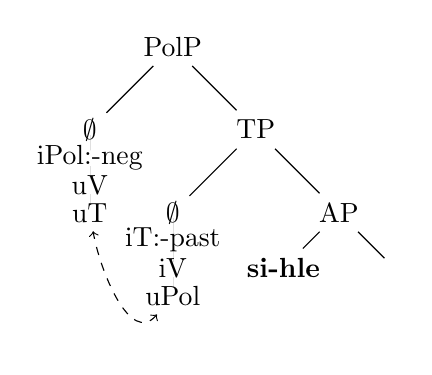
\begin{tikzpicture}[
sibling distance=6em,
level distance=3em]
\node (root) at (0,0) {PolP}
			child { node  {$\emptyset$} [sibling distance=8em, level distance=1em]
				child { node {iPol:-neg} [line width=.001mm, sibling distance=8em, level distance=1em]
					child { node {uV}
						child { node (pol){uT}}}}}
			child {node {TP}[sibling distance=6em, level distance=3em]
				child { node {$\emptyset$}[sibling distance=8em, level distance=1em]
						child { node {iT:-past}  [line width=.001mm, sibling distance=8em, level distance=1em]
							child { node { iV}
								child { node (t){uPol}}}}}
				child { node {AP}[sibling distance=4em, level distance=2em] 
						child { node  {\textbf{si-hle}}}
						child { node {}}}};
%\draw (V) [->]to[out=280,in=270] (vt);
%\draw[->, dashed] (pol) to[out=230,in=280] (c);

\draw[<->, dashed] (t) to[out=230,in=280] (pol);
%\draw[<-,dashed] (pol) to[out=230,in=100] (0, -4);

%\draw[<-, dashed] (V) to[out=250,in=280] (-1.5,-4.5);
%\draw[dashed] (pol) to[out=250,in=100] (-1.5,-4.5);

%\draw[dashed] (t) to[out=250,in=280] (-1.5,-3);
%\draw[dashed] (c) to[out=220,in=100] (-1.5,-3);
\end{tikzpicture}




\begin{exe}
\ex
\end{exe}

\todo[inline]{Tree commented out due to compile problems}

% \begin{tikzpicture}[
% sibling distance=6em,
% level distance=2em]
% \node (root) at (0,0) {PolP}
% 			child { node  {\textbf{a}} [sibling distance=8em, level distance=1em]
% 				child { node {iPol:+neg} [line width=.001mm, sibling distance=8em, level distance=1em]
% 					child { node {uV}
% 						child { node {uT}
% 							child { node (pol){uVerb}}}}}}
% 			child {node {TP}[sibling distance=8em, level distance=5em] 
% 				child { node {T}[sibling distance=4em, level distance=2em] 
% 					child { node (vt) {\textbf{si-$\emptyset$_i}} }
% 					child { node {$\emptyset$}  [ sibling distance=8em, level distance=1em]
% 						child { node {iT:-past}  [line width=.001mm, sibling distance=8em, level distance=1em]
% 							child { node { iV: -V}
% 								child { node (t){uPol}}}}}}
% 				child { node {VP}[sibling distance=4em, level distance=2em] 
% 						child { node  {t_i}[sibling distance=8em, level distance=1em]
% 							child { node (V){iVerb} [line width=.001mm]}}
% 						child { node {AP}
% 							child { node {\textbf{si-hle}}}
% 							child { node {}}}}};
% %\draw (V) [->]to[out=280,in=270] (vt);
% %\draw[->, dashed] (pol) to[out=230,in=280] (c);
% 
% \draw[<-, dashed] (t) to[out=230,in=280] (-2, -4);
% \draw[<-,dashed] (pol) to[out=230,in=100] (-2, -4);
% 
% \draw[<-, dashed] (V) to[out=250,in=280] (-1.5,-4.5);
% \draw[dashed] (pol) to[out=250,in=100] (-1.5,-4.5);
% 
% %\draw[dashed] (t) to[out=250,in=280] (-2,-3);
% %\draw[dashed] (c) to[out=220,in=100] (-2,-3);
% \end{tikzpicture}










\begin{exe}
\ex
\end{exe}

\todo[inline]{Tree commented out due to compile problems}

% \begin{tikzpicture}[
% sibling distance=8em,
% level distance=3em]
% \node (root) at (0,0) {PolP}
% 			child { node  {$\emptyset$} [sibling distance=8em, level distance=1em]
% 				child { node {iPol:-neg} [line width=.001mm, sibling distance=8em, level distance=1em]
% 					child { node {uV}
% 							child { node (pol){uT}}}}}
% 			child {node {TP}[sibling distance=8em, level distance=3em] 
% 				child { node {T}[sibling distance=4em, level distance=2em] 
% 					child { node (vt) {be_j-\textbf{si-$\emptyset$_i}} }
% 					child { node {$\emptyset$}  [ sibling distance=8em, level distance=1em]
% 						child { node {iT:+past}  [line width=.001mm, sibling distance=8em, level distance=1em]
% 							child { node { iV: -V}
% 								child { node {uVerb}
% 									child { node (t){uPol}}}}}}}
% 				child { node {VP}[sibling distance=4em, level distance=2em] 
% 						child { node  {t_i}[sibling distance=8em, level distance=1em]
% 							child { node (V){iVerb} [line width=.001mm]}}
% 				child { node {AuxP}
% 					child { node {t_j}}
% 						child { node {AP}
% 							child { node {\textbf{si-hle}}}
% 							child { node {}}}}}};
% \draw (V) [<-, dashed]to[out=280,in=270] (t);
% %\draw[->, dashed] (pol) to[out=230,in=280] (c);
% 
% \draw[<-, dashed] (t) to[out=230,in=280] (-2, -4);
% \draw[<-,dashed] (pol) to[out=230,in=100] (-2, -4);
% 
% %\draw[<-, dashed] (V) to[out=250,in=280] (-1.5,-4.5);
% %\draw[dashed] (pol) to[out=250,in=100] (-1.5,-4.5);
% 
% %\draw[dashed] (t) to[out=250,in=280] (-1.5,-3);
% %\draw[dashed] (c) to[out=220,in=100] (-1.5,-3);
% \end{tikzpicture}





\begin{exe}
\ex
\end{exe}

\todo[inline]{Tree commented out due to compile problems}

% \begin{tikzpicture}[
% sibling distance=8em,
% level distance=3em]
% \node (root) at (0,0) {PolP}
% 			child { node  {$\emptyset$} [sibling distance=8em, level distance=1em]
% 				child { node {iPol:+neg} [line width=.001mm, sibling distance=8em, level distance=1em]
% 					child { node {uV}
% 						child { node {uVerb}
% 							child { node (pol){uT}}}}}}
% 			child {node {TP}[sibling distance=8em, level distance=3em] 
% 				child { node {T}[sibling distance=4em, level distance=2em] 
% 					child { node (vt) {be_j-\textbf{si-$\emptyset$_i}} }
% 					child { node {\textbf{nga}}  [ sibling distance=8em, level distance=1em]
% 						child { node {iT:+past}  [line width=.001mm, sibling distance=8em, level distance=1em]
% 							child { node { iV: -V}
% 								child { node {uPol}
% 									child { node (t) {uVerb}}}}}}}
% 				child { node {VP}[sibling distance=4em, level distance=2em] 
% 						child { node  {t_i}[sibling distance=8em, level distance=1em]
% 							child { node (V){iVerb} [line width=.001mm]}}
% 				child { node {AuxP}
% 					child { node {t_j}}
% 						child { node {AP}
% 							child { node {\textbf{si-hle}}}
% 							child { node {}}}}}};
% %\draw (V) [->]to[out=280,in=270] (vt);
% %\draw[->, dashed] (pol) to[out=230,in=280] (c);
% 
% \draw[<-, dashed] (t) to[out=230,in=280] (-2, -4);
% \draw[<-,dashed] (pol) to[out=230,in=100] (-2, -4);
% 
% \draw[<-, dashed] (V) to[out=250,in=280] (-1,-6);
% \draw[dashed] (pol) to[out=250,in=100] (-1,-6);
% 
% %\draw[dashed] (t) to[out=250,in=280] (-1.5,-3);
% %\draw[dashed] (c) to[out=220,in=100] (-1.5,-3);
% \end{tikzpicture}



\subsubsection{Multiple subject marking}

A counter proposal to the one presented in \S3.2 would be one that uses \bee as an additional verbal element which triggers the presence of the second subject marking, instead of positing a null verbal element. In this scenario, \bee is generated where our null verbal element is (see (15) and (17)), causing a second agreement marker to appear, and in the case of (17), taking \nga as a suffix. The argument would then have \bee moving up to a higher node in order to get the correct surface ordering.

One reason why this solution is not implemented in this paper is evidence that \bee can generate its own subject marking independent from and in addition to that seen in  (13a-b). This third subject marking is shown in (18d).



\begin{exe}
\ex \begin{xlist}
\ex \gll  \textit{yenza} \textit{isi-lwane} \textit{si-be-si-hle}\\
       make 7-lion 7.{\sc sm}-be.{\sc pst}-7.{\sc sm}-pretty\\
    \glt `Make the lion be pretty'

\ex \gll  \textit{yenza} \textit{isi-lwane} \textit{si-be-$\emptyset$-nga-nhle}\\
       make 7-lion 7.{\sc sm}-be.{\sc pst}-$\emptyset$-{\sc neg}-pretty\\
    \glt `Make the lion not be pretty' 
\ex \gll  \textit{yenza} \textit{isi-lwane} \textit{si-be-si-$\emptyset$-nga-nhle}\\
       make 7-lion 7.{\sc sm}-be.{\sc pst}-7.{\sc sm}-$\emptyset$-{\sc neg}-pretty\\
    \glt `Make the lion not be pretty' 
\ex \gll  \textit{yenza} \textit{isi-lwane} \textit{si-be-si-$\emptyset$-nga-si-hle}\\
       make 7-lion 7.{\sc sm}-be.{\sc pst}-7.{\sc sm}-$\emptyset$-{\sc neg}-7.{\sc sm}-pretty\\
    \glt `Make the lion not be pretty' 
\ex \gll  *\textit{yenza} \textit{isi-lwane} \textit{si-be-$\emptyset$-nga-si-hle}\\
       make 7-lion 7.{\sc sm}-be.{\sc pst}-$\emptyset$-{\sc neg}-7.{\sc sm}-pretty\\
    \glt `Make the lion not be pretty' 
\end{xlist}
\end{exe}

Additional evidence that \bee generates its own independent subject marking is given by Sibanda, who provides the following forms (Sibanda 2004).

\begin{exe}
\ex \begin{xlist} 
\ex \textit{zibe zihamba} \ensuremath\longrightarrow \textit{bezihamba} `they were walking/moving/going'\\
\textit{sibe sikhala} \ensuremath\longrightarrow \textit{besiskhala} `it was crying'

\ex \textit{ibe ihamba} \ensuremath\longrightarrow \textit{ibihamba} `it was walking'\\
\textit{ube ekhala} \ensuremath\longrightarrow \textit{ubekhala} `s/he was crying'
\end{xlist}
\end{exe}

The evidence provided in this section makes it unlikely that the double subject marking can be accounted for by \bee alone. 



\subsubsection{Selection}. 

Now that more than one type of predicate has been introduced, the selectional properties of TP need to be discussed. One benefit of an approach which accounts for the null verbal projection with respect to repair is that the selectional properties of TP do not then need to account for this phenomenon. Rather, we can posit that present tense adjectival TP selects for AP and past tense adjectival TP selects for a BeP, which in turn selects an AP.\footnote{BeP is a convenient name for the projection most often realized as \textit{be}, see \S3.3.1 for more discussion of \textit{be}.}
\\

\textbf{Selection}\footnote{For a full list of lexical entries, see the appendix.}
\begin{exe}
\ex TP\textsubscript{Adj, Past}: =AP, T -V +Past
\ex TP\textsubscript{Adj, Present}: =BeP, +Adj, T -V -Past
\ex BeP: =AP, Be 
\end{exe}

If instead of this repair scheme, the motivation for the null verb was accounted for purely via selection, the account would run into troubles. Most importantly, it can be see that the null verb appears in either the presence of negation or past tense. Thus if this scenario were accounted for purely through selection, both negative polarity and past tense would select for a null verbal element. With this set up, a sentence like (13b) would instead appear as in (23), which is ungrammatical.

\begin{exe}
\ex \gll *\textit{isi-lwane} \textit{be-si-$\emptyset$-si-$\emptyset$-{\bf nga}-si-hle}\\
       7-lion be.{\sc pst}-7.{\sc sm}-$\emptyset$-7.{\sc sm}-$\emptyset$-{\sc neg}-7.{\sc sm}-pretty\\
    \glt `The lion wasn't pretty' 
\end{exe}

Rather, it seems that a single verbal component is enough to satisfy the requirements of both the NegP and the past tense. This observation fits nicely with the system of Agreement adopted in this paper.

It is worth noting as well that \nga is the only overt realization of tense which appears in non-verbal clauses. The realizations of non-verbal past tense are specifically designed this way in Table 6 in order to prevent the appearance of other overt final vowels appearing before adjectival predicates. The featural specifications for realizations of tense are repeated in Tables 6-8 for convenience. 


\begin{table}
\caption{Realizations of Past Tense} %title of the table 
\centering % centering table 
\begin{tabular}{c| rr|r|r} % creating eight columns 
\hline %inserting double-line 
 &\multicolumn{2}{c}{-nga-}& \multicolumn{1}{|c}{-e-}& \multicolumn{1}{|c}{$\emptyset$} \\ [0.5ex] 
\hline % inserts single-line 
Neg & + & + & - & -\\ % Entering row contents 
Verbal & + & - & +& -\\[1ex] % [1ex] adds vertical space 
\hline % inserts single-line 
\end{tabular} 
\label{tab:hresult} 
\end{table} 





\begin{table}
\caption{Realizations of Present Tense} %title of the table 
\centering % centering table 
\begin{tabular}{c| r|r|rr} % creating eight columns 
\hline %inserting double-line 
 &\multicolumn{1}{c}{-i-}& \multicolumn{1}{|c|}{-a-}& \multicolumn{2}{|c}{$\emptyset$} \\ [0.5ex] 
\hline % inserts single-line 
Neg & + & - & + & -\\ % Entering row contents 
Verbal & + & + & -& -\\[1ex] % [1ex] adds vertical space 
\hline % inserts single-line 
\end{tabular} 
\label{tab:hresult} 
\end{table} 



\begin{table}
\caption{Realizations of Future Tense} %title of the table 
\centering % centering table 
\begin{tabular}{c| rrrr} % creating eight columns 
\hline %inserting double-line 
 &\multicolumn{4}{c}{-za-} \\ [0.5ex] 
\hline % inserts single-line 
Neg & + & + & - & -\\ % Entering row contents 
Verbal & + & - & +& -\\[1ex] % [1ex] adds vertical space 
\hline % inserts single-line 
\end{tabular} 
\label{tab:hresult} 
\end{table} 


\subsection{Future tense adjectival predicates}

This section looks at the way future tense adjectival predicates are formed in Ndebele. Though these forms show slightly different surface structure than the present and past tense counterparts, they still are able to fit into the system otherwise outlined in this paper.


\begin{exe}
\ex \begin{xlist}
\ex \gll \textit{isi-lwane} \textit{si-za-be} \textit{si-$\emptyset$-si-hle}\\
       7-lion 7.{\sc sm}-FUT-be.{\sc pst} 7.{\sc sm}-$\emptyset$-7.{\sc sm}-pretty\\
    \glt `The lion will be pretty' 

\ex \gll \textit{isi-lwane} \textit{si-za-be} \textit{si-$\emptyset$-nga-si-hle}\\
       7-lion 7.{\sc sm}-FUT-be.{\sc pst} 7.{\sc sm}-$\emptyset$-{\sc neg}-7.{\sc sm}-pretty\\
    \glt `The lion will not be pretty' 
\end{xlist}
\end{exe}

The difference between future tense adjectival predicates and their counterparts is the future morpheme \textit{-za-}. This morpheme, which originally was an independent verb, has become grammaticalized to serve as the future tense marker, though presumably due to its historical origins it does so outside of the canonical TP position (Sibanda 2004). The trees in (25) and (26) represent the sentences in (24a-b).



\begin{exe}
\ex
\end{exe}
\todo[inline]{tree commented out due to compile problems}
% \begin{tikzpicture}[
% sibling distance=6em,
% level distance=3em]
% \node (root) at (0,0) {PolP}
% 			child { node  {$\emptyset$} [sibling distance=8em, level distance=1em]
% 				child { node {iPol:-neg} [line width=.001mm, sibling distance=8em, level distance=1em]
% 					child { node {uV}
% 							child { node (pol){uT}}}}}
% 				child { node {ZP}
% 					child { node {si-za}}
% 			child {node {TP}[sibling distance=8em, level distance=3em] 
% 				child { node {T}[sibling distance=4em, level distance=2em] 
% 					child { node (vt) {\textbf{be_j-si-$\emptyset$_i}} }
% 					child { node {$\emptyset$}  [ sibling distance=8em, level distance=1em]
% 						child { node {iT:+past}  [line width=.001mm, sibling distance=8em, level distance=1em]
% 							child { node { iV: -V}
% 								child { node {uVerb}
% 									child { node (t){uPol}}}}}}}
% 				child { node {VP}[sibling distance=4em, level distance=2em] 
% 						child { node  {t_i}[sibling distance=8em, level distance=1em]
% 							child { node (V){iVerb} [line width=.001mm]}}
% 			child { node {AuxP}
% 				child { node {t_j}}
% 						child { node {AP}
% 							child { node {\textbf{si-hle}}}
% 							child { node {}}}}}}};
% \draw (V) [<-, dashed]to[out=280,in=270] (t);
% %\draw[->, dashed] (pol) to[out=230,in=280] (c);
% 
% \draw[<-, dashed] (t) to[out=230,in=280] (-2, -4);
% \draw[<-,dashed] (pol) to[out=230,in=100] (-2, -4);
% 
% %\draw[<-, dashed] (V) to[out=250,in=280] (-1.5,-4.5);
% %\draw[dashed] (pol) to[out=250,in=100] (-1.5,-4.5);
% 
% %\draw[dashed] (t) to[out=250,in=280] (-1.5,-3);
% %\draw[dashed] (c) to[out=220,in=100] (-1.5,-3);
% \end{tikzpicture}




\begin{exe}
\ex
\end{exe}
\todo[inline]{Tree commented out due to compile problems}
% \begin{tikzpicture}[
% sibling distance=8em,
% level distance=3em]
% \node (root) at (0,0) {PolP}
% 			child { node  {$\emptyset$} [sibling distance=8em, level distance=1em]
% 				child { node {iPol:+neg} [line width=.001mm, sibling distance=8em, level distance=1em]
% 					child { node {uV}
% 						child { node {uVerb}
% 							child { node (pol){uT}}}}}}
% 				child { node {ZP}
% 					child { node {si-za}}
% 			child {node {TP}[sibling distance=8em, level distance=3em] 
% 				child { node {T}[sibling distance=4em, level distance=2em] 
% 					child { node (vt) {\textbf{be_j-si-$\emptyset$_i}} }
% 					child { node {\textbf{nga}}  [ sibling distance=8em, level distance=1em]
% 						child { node {iT:+past}  [line width=.001mm, sibling distance=8em, level distance=1em]
% 							child { node { iV: -V}
% 								child { node {uPol}
% 									child { node (t) {uVerb}}}}}}}
% 				child { node {VP}[sibling distance=4em, level distance=2em] 
% 						child { node  {t_i}[sibling distance=8em, level distance=1em]
% 							child { node (V){iVerb} [line width=.001mm]}}
% 			child { node {AuxP}
% 				child { node {t_j}}
% 						child { node {AP}
% 							child { node {\textbf{si-hle}}}
% 							child { node {}}}}}}};
% %\draw (V) [->]to[out=280,in=270] (vt);
% %\draw[->, dashed] (pol) to[out=230,in=280] (c);
% 
% \draw[<-, dashed] (t) to[out=230,in=280] (-2, -4);
% \draw[<-,dashed] (pol) to[out=230,in=100] (-2, -4);
% 
% \draw[<-, dashed] (V) to[out=250,in=280] (-1,-6);
% \draw[dashed] (pol) to[out=250,in=100] (-1,-6);
% 
% %\draw[dashed] (t) to[out=250,in=280] (-1.5,-3);
% %\draw[dashed] (c) to[out=220,in=100] (-1.5,-3);
% \end{tikzpicture}




\subsubsection{Accounting for \bee}

In \S3.2 on past tense adjectival predicates we accounted for the presence of the auxiliary verb \bee by stipulating that it is selected for by a past tense non-verbal tense node. In  examples (24a-b), however, we find \bee appearing with a semantically future tense clause. Thus, some explanation needs to be given in order to make sense of the distribution of \textit{be}. On the account presented here the presence of \bee is strictly selected for by a past tense non-verbal tense node. Thus, more needs to be said about ZP.
In the analysis above, the node ZP has been introduced as a sort of tense node (which makes it an available to be selected by PolP), which itself selects for a non-future tense node. The ZP tense node differs from regular TPs in a few crucial ways. The first is that while it carries a +/-V feature, in place of the binary +/-past feature, it simply has a +FUT feature. The +/-V feature is crucial to this node in that it dictates what sort of tense node is selected by the ZP. Verbal clause ZPs select a -past TP, while non-verbal clause ZPs select for a past tense node, as seen in the examples above. This selection of the past tense node is what, in turn, allows us to explain the presence of \bee where it would not normally be expected (outside of a semantically past tense clause). 


























\section{Imperatives}

This section examines how imperatives are formed and negated in Ndebele. This particular phenomenon will be examined because it is another case in which the negative affix \nga appears pre-verbally in the surface structure. Once again the proposal outlined in the preceding sections will be applied to this phenomenon.

The basic form of the imperative appears in (27)-(28).


\begin{exe}
\ex \begin{xlist}
\ex \gll \textit{hamb-a}\\
        go-FV\\
    \glt `Go!'

\ex \gll \textit{u-\textbf{nga}-hamb-i}\\
        1.{\sc sm}-{\sc neg}-go-{\sc neg}\\
    \glt `Don't Go!'
\end{xlist}
\end{exe}




\begin{exe}
\ex \begin{xlist}
\ex \gll \textit{val-a} \textit{um-ngango}\\
        close-FV 3-door\\
    \glt `Close the door!'


\ex \gll \textit{u-nga-val-i} \textit{um-ngango}\\
        1.{\sc sm}-NEG-close-NEG 3-door\\
    \glt `Don't close the door!'
\end{xlist}
\end{exe}

As mentioned above, the negative affix \nga appears in the negated forms in (27b) and (28b). What is puzzling about these facts, given the descriptions and analyses so far, is why \nga should be the affix that negates such sentences, as up to this point \nga has only appeared either in past tense clauses, or future adjectival clauses. While the use of \nga in (27b) and (28b) does not fit the pattern we have seen so far, it could of course be part of a larger pattern not analyzed in this paper.

Aside from these distributional concerns, the form of the negative imperatives above seems completely amenable to the analysis developed here. By positing that in these situations too there is a null verbal element which takes both a subject marker and negative suffix, the surface string can be brought into the analysis. The tree for this is given in (29).


\begin{exe}
\ex
\end{exe}
\todo[inline]{tree commented out due to compile problems}
% \begin{tikzpicture}[
% sibling distance=6em,
% level distance=3em]
% \node (root) at (0,0) {PolP}[sibling distance=10em, level distance=3em]
% 			child { node  {$\emptyset$} [sibling distance=8em, level distance=1em]
% 				child { node {iPol:+neg} [line width=.001mm, sibling distance=8em, level distance=1em]
% 					child { node {uV}
% 						child { node {uVerb}
% 							child { node (pol){uT}}}}}}
% 			child {node {TP}[sibling distance=8em, level distance=3em] 
% 				child { node {T}[sibling distance=4em, level distance=2em] 
% 					child { node (vt) {\textbf{u-$\emptyset$_i}} }
% 					child { node {\textbf{nga}}  [ sibling distance=8em, level distance=1em]
% 						child { node {iT:-past}  [line width=.001mm, sibling distance=8em, level distance=1em]
% 							child { node { iV: -V}
% 									child { node (t) {uPol}}}}}}
% 				child { node {VP}[sibling distance=6em, level distance=3em] 
% 						child { node  {t_i}[sibling distance=8em, level distance=1em]
% 							child { node (V){iV} [line width=.001mm]}}
% 						child { node {TP}[sibling distance=8em, level distance=4em] 
% 				child { node {T}[sibling distance=4em, level distance=2em] 
% 					child { node (vt) {\textbf{$\emptyset$-hamb_j}} }
% 					child { node {\textbf{i}}  [ sibling distance=8em, level distance=1em]
% 						child { node {iT:-past}  [line width=.001mm, sibling distance=8em, level distance=1em]
% 							child { node {iV: +V}
% 									child { node (t2) {uPol}}}}}}
% 				child { node {VP}[sibling distance=4em, level distance=2em] 
% 						child { node  {t_j}[sibling distance=8em, level distance=1em]
% 							child { node (V2){iV} [line width=.001mm]}}
% 						child { node {}}}}}};
% %\draw (V) [->]to[out=280,in=270] (vt);
% %\draw[->, dashed] (pol) to[out=230,in=280] (c);
% 
% \draw[<->, dashed] (t) to[out=230,in=280] (pol);
% \draw[<-,dashed] (pol) to[out=230,in=280] (t2);
% 
% \draw[<-, dashed] (V) to[out=250,in=280] (-2,-4.5);
% \draw[dashed] (pol) to[out=250,in=100] (-2,-4.5);
% 
% %\draw[dashed] (t) to[out=250,in=280] (-1.5,-3);
% %\draw[dashed] (c) to[out=220,in=100] (-1.5,-3);
% 
% %second clause
% 
% %\draw (V) [->]to[out=280,in=270] (vt);
% %\draw[->, dashed] (pol2) to[out=230,in=280] (c2);
% 
% %\draw[->, dashed] (t2) to[out=230,in=280] (pol);
% %\draw[<-,dashed] (pol) to[out=230,in=100] (3, -8.7);
% 
% %\draw[<-, dashed] (V2) to[out=250,in=280] (-1.5,-4.5);
% %\draw[dashed] (pol2) to[out=250,in=100] (-1.5,-4.5);
% 
% %\draw[dashed] (t2) to[out=250,in=280] (3.6,-8.8);
% %\draw[dashed] (c2) to[out=220,in=100] (3.6,-8.8);
% 
% 
% \end{tikzpicture}

The motivation for such an analysis seems to be primarily lacking in the case of imperatives. Throughout this paper it has been the tense node  (or the tense auxiliary) which has selected for a null verbal element. In the case of imperative sentences like the one above, it is unclear what would motivate the tense node to select for a null verbal element, bringing imperatives in line with the rest of our analysis. Thus it is unclear whether imperative sentences should be analyzed under the same rubric as the other examples in this paper, or whether they are better described as a separate phenomenon.

\section{Conclusions}

In this paper negation in Ndebele has been examined across many different subcategories of the language. In \S1 the distribution of negative morphemes in Ndebele was captured using a complex featural system and bi-directional agreement. In \S2 a proposal for the clausal structure of negative sentences in Ndebele was proposed with respect to simple tense past and present verbal predicates. In the following sections this analysis was extended to cases where the negative affix \nga appears pre-verbally instead of post-verbally, as it does in the simple tense sentences. 

When adjectival predicates were examined, it was seen that by positing a null verbal projection which hosts both subject agreement and the polarity sensitive tense node \textit{-nga-}, it was possible to account for seemingly pre-fixal \nga and to explain previously unaccounted for double subject marking in certain adjectival predicates. In the last section, the analysis was extended to imperatives, again an area which exhibits pre-verbal \textit{-nga-}. With respect to this phenomenon, however, the motivation for extending the analysis was significantly weaker, enough to call into question the application of the null verbal element as a solution for pre-verbal \textit{-nga-}.

More detailed questions still need to be answered including what the proper analysis of imperatives should be. That is, should they be treated with approach outlined in this paper, or is this phenomenon merely similar from the perspective of surface structure? Another troubling feature of this analysis is the lack of evidence for the negative affix \ii to appear preverbally. The claim made in this paper is that both \nga and \ii are generated in a tense sensitive tense node. All things being equal, one would assume that finding \nga pre-verbally would be an indicator that \ii should appear there as well, though there might be confounding variables at work which prevent \ii from surfacing overtly in this position.\footnote{See Buell (2004)  for some evidence that \ii might indeed appear pre-verbally}

This paper is intended as a contribution to the field of Bantu linguistics and to studies on polarity. As this paper presents an alternate analysis of polarity and tense in Ndebele, future research should be able to ascertain whether or not aspects of this analysis, such as the treatment of final vowels as tense nodes, can be extended to other Nguni or Bantu languages. Other languages which exhibit bipartite negation would also serve as targets for comparison with respect to the analysis of bipartite negation developed here. Such comparisons and questions are left for future research. 
\vspace{5 mm}

\section*{Appendix}

This appendix shows the selectional properties of the various  syntactic constructions used in this paper.

PolP: =TP, Pol
\\
ZP\textsubscript{+V}: =TP PRES +V, T 
\\
ZP\textsubscript{-V}: =TP PAST -V, T 
\\
TP\textsubscript{V}: =VP, T +V
\\
TP\textsubscript{Adj, Past}: =AP, T -V +Past
\\
TP\textsubscript{Adj, Present}: =BeP +Adj, T -V -Past
\\
Be: =AP, Be 
\\
TP\textsubscript{-Main}: =BeP -M, T -M
\\
BeP\textsubscript{-Main}: =PolP, Be -M


\section*{Abbreviations}

\sc{neg} \quad negation
\\
Numbers \quad signify noun class (ie 1, 7)
\\
\sc{sm} \quad subject marker
\\
\sc{prs} \quad present tense
\\
\sc{cop} \quad copula
\\
\sc{pst} \quad past tense
\\
\sc{ep} \quad epenthetic (vowel)
\\
\sc{fut} \quad future tense
\\
\sc{fv} \quad final vowel


\begin{verbatim}
\nocite{*}

Bjorkman, Bronwyn. 2011. Be-ing default: The morphosyntax of auxiliaries. Doctoral

 Dissertation, Massachusetts Institute of Technology, Cambridge, MA.
\\
\\
Boskovic, Z. 2007. On the locality and motivation of Move and Agree: An even more

 minimal theory. \textit{Linguistic Inquiry 38}: 589-644.
\\
\\
Buell, Lester C. 2004. \textit{The Zulu Verb Within the Constraints of the LCA}. Accessed 

online 5/28/2013.
\\
\\
Buell, Lester C. 2005. \textit{Issues in Zulu Verbal Morphosyntax} (Doctoral dissertation). 

Accessed online 5/28/2013.
\\
\\
Chomsky, Noam. 2001. Derivation by phase. In \textit{Ken Hale: A life in language}, ed.

 M. Kenstowicz, 1-52. Cambridge: MIT Press.
\\
\\
Hall, Linda. 2005. The -be Relative Tenses of Zulu. Doctoral Dissertation, 

University of Pretoria.
\\
\\
Khumalo, J.S.M. 1981. Zulu tonology, part 1. \textit{African Studies 40}(2), 53-130.
\\
\\
Khumalo, J.S.M. 1982. Zulu tonology, part 2. \textit{African Studies 41}(1), 3-126.
\\
\\
Rizzi, Luigi. 1989. \textit{Relativised Minimality}. Cambridge, MA: The MIT Press.
\\
\\
Sibanda, Galen. 2004. \textit{Verbal Phonology and Morphology of Ndebele} 

(Doctoral dissertation). Accessed online 5/28/2013.
\\
\\
Zeijlstra, Hedde. 2010. There is only one way to agree. Talk given at GLOW 33, 

Wroclaw, Poland.
\end{verbatim}





\section*{Abbreviations}
\section*{Acknowledgements}

\printbibliography[heading=subbibliography,notkeyword=this]

\end{document}